\documentclass{article}
\usepackage[utf8]{inputenc}

\usepackage{problems}
\usepackage{graphicx}
\usepackage{todonotes}
\usepackage{enumitem}

\graphicspath{ {./images/} }

\NewTasksEnvironment[label=\Alph*]{tasks2}[\task]

\newcommand{\degree}{\ensuremath{^{\circ}}}
\renewcommand{\angle}{\measuredangle}

\begin{document}
\section{Easy}
\begin{problem}
What is the smallest integer greater than $1$ which is both a square and a cube?
\end{problem}
%%%%%%%\answer{64}

\begin{problem}
What is the smallest positive, odd integer that is not a prime and not a square?
\end{problem}
%%%%%%%\answer{15}


\begin{problem}
How many integers are there between $10$ and $1000$ that stay the same when the order of their digits is reversed?
\end{problem}
%%%%%%%\answer{99}

\begin{problem}
Assuming that all its angles are $90\degree$, what is the perimeter of the following shape? \\
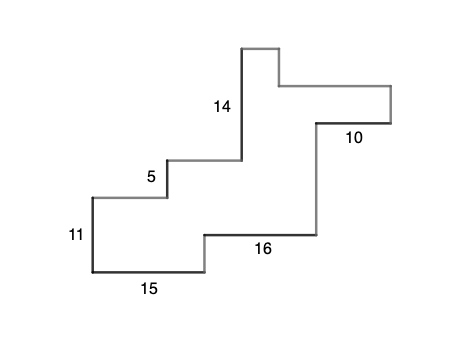
\includegraphics[width = 8cm]{img10.png}
\end{problem}
%%%%%%%\answer{142}

\begin{problem}
The sum of five consecutive integers equals the sum of the three next bigger numbers. What is the biggest of these eight numbers?
\end{problem}
\begin{tasks}(5)
\task 4
\task 8
\task 9
\task 11
\task 12
\end{tasks}
%%%%%%%%\answer{d)}

\begin{problem}
On a cube, we label each of its faces and vertices with $1$ and each edge with $-1$. What is the total sum of the labels?
\end{problem}
\begin{tasks}(6)
\task 0
\task 2
\task 4
\task 6
\task 8
\end{tasks}
%%%%%%%\answer{b)}

\newpage

\begin{problem}
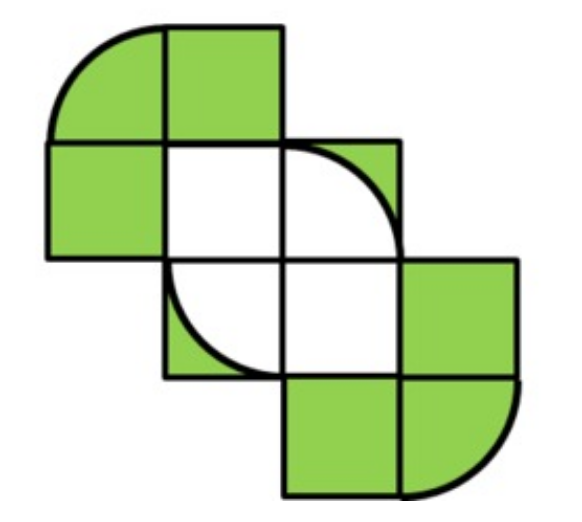
\includegraphics[width=150pt]{img5} \\
Using her compass, Rada drew this figure on a grid paper. If the side length of one small square is $2$, what is the green area?
\end{problem}
\begin{tasks}(5)
\task $12$
\task $16$
\task $16 + 2\pi$
\task $24$
\task $24 + 2\pi$
\end{tasks}
%%%%%%%\answer{d)}

\begin{problem}
Tim forgot the last five letters of his password. He only remembers that each letter is one of $I$, $M$ or $O$. How many possibilities does he have to take into consideration? \\
\end{problem}
\begin{tasks}(5)
\task 15
\task 20
\task 120
\task 125
\task 243
\end{tasks}
%%%%%%%%\answer{e)}

\begin{problem}
Which statements about the following configuration must certainly hold, assuming that $M$ is the center of the semicircle?\\
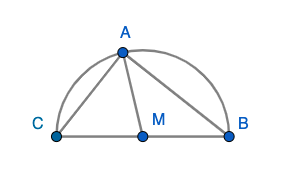
\includegraphics[width=200pt]{img1}
\begin{tasks2}(2)
\task $\angle CAM = \angle ABC$
\task $\angle AMC = 2\angle ABC$
\task $\angle ACB + \angle ABC = 90\degree$
\task $Area(ACM) = Area(AMB)$
\end{tasks2}
\end{problem}
%%%%%%%\answer{B, C and D}

\begin{problem}
The number $323$ is...
\begin{tasks2}(2)
\task a prime
\task a square
\task the difference of two primes
\task the difference of two squares
\end{tasks2}
\end{problem}
%%%%%%%\answer{D}

%%
\newpage
%%
\section{Medium}

\begin{problem}
If the diagonal of square $A$ is $16$ times as large as the perimeter of square $B$, how many times as large is its area?
\end{problem}
%%%%%%%\answer{2048}

\begin{problem}
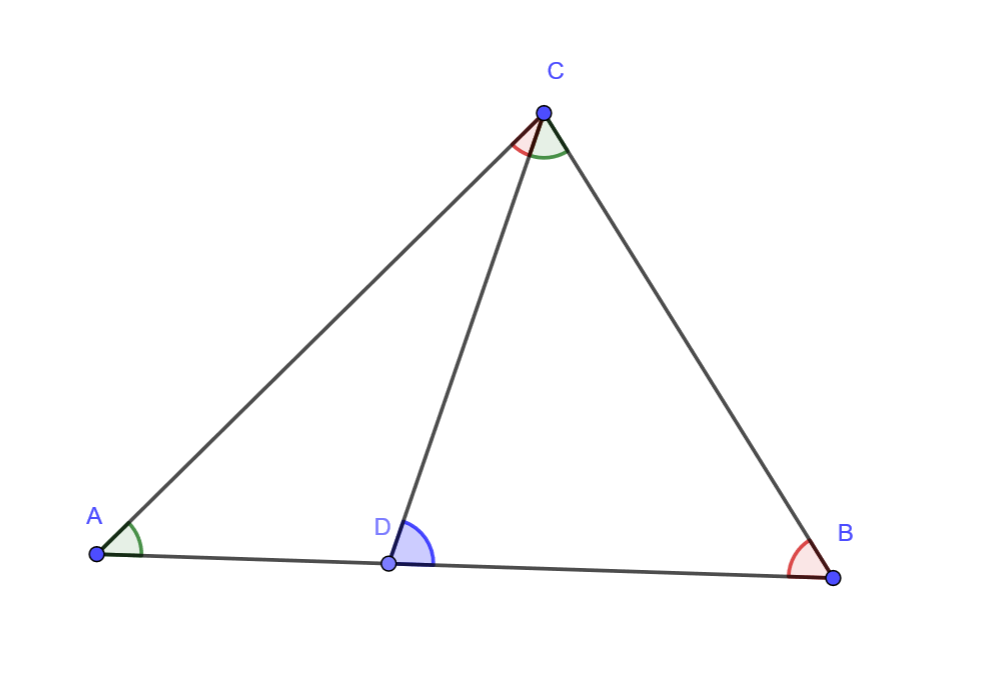
\includegraphics[width=250pt]{img11.png} \\
Suppose that, in the diagram above, the angles $\angle DAC$ and $\angle DCB$ (both highlighted green) are $45^{\circ}$ and that the angle $\angle CBD$ is twice as large as the angle $\angle ACD$ (both highlighted red). How many degrees is the blue angle $\angle BDC$?
\end{problem}

\begin{problem}
Paul made less than $200$ cookies and now wishes to distribute them into paper bags, such that each bag has exactly the same number of cookies. Sadly, this never seems to work out: If he wants to distribute them into $5$ bags, there are four cookies left. The same thing happens if he wants to distribute them into $6$ bags. If he wants to have $7$ bags, there are $3$ cookies left. How many cookies did Paul make in total?
\end{problem}
%%%%%%%\answer{94}

\begin{problem}
If a right angled triangle has a side of length $15$ and a side of length $12$, what is its smallest possible area?
\end{problem}
%%%%%%%\answer{54}

\begin{problem}
What integer has the property that if you square it and subtract $49$ you get the same number as if you first subtract $49$ and then square it?
\end{problem}
%%%%%%%\answer{25}

\begin{problem}
Henning's favourite ice cream store offers $8$ different flavours. Henning wants to buy three scoops of ice cream which are not all of the same flavour. How many possibilities does he have to do this? \\
\emph{Remark: The order of the flavours doesn't matter.}
\end{problem}
%%%%%%%\answer{112}
\newpage

\begin{problem}
What is the remainder of $2^2 \times 3^3 \times 5^5 \times 7^7$ when divided by $8$?
\end{problem}
\begin{tasks}(5)
\task 2
\task 3
\task 4
\task 5
\task 7
\end{tasks}
%%%%%%%\answer{c)}

\begin{problem}
Given is a square $ABCD$ in the plane. How many squares are there that share exactly two vertices with $ABCD$?
\end{problem}
\begin{tasks}(5)
\task 4
\task 6
\task 8
\task 12
\task 16
\end{tasks}
%%%%%%%\answer{d)}

\begin{problem}
Julia and Florian independently think of an integer between $1$ and $10$. Julia says: "No matter what number you chose: If we compute the product of our two numbers, it will not contain the digit $6$.". Florian says: "Alright, then the sum of our numbers must be $14$." What is Florian's number?
\end{problem}
\begin{tasks}(5)
\task 4
\task 5
\task 6
\task 8 
\task 9
\end{tasks}
%%%%%%%\answer{e)}

\begin{problem}
Which is the smallest integer $n > 2$ such that $(2^2-1)\cdot(3^2-1) \cdot \ldots \cdot (n^2-1)$ is a square number?
\end{problem}
\begin{tasks}(5)
\task 7
\task 8
\task 9
\task 11
\task 12
\end{tasks}
%%%%%%%\answer{b)}

\begin{problem}
Tanish thinks of an integer $1\leq n \leq 100$ and Marco wants to guess the number. After each guess, Tanish tells him whether his guess was correct, too small or too big. Marco wins as soon as he guesses the correct number. What is the smallest number of guesses that can guarantee Marco to win, assuming he guesses smartly?
\begin{tasks}(5)
\task 4
\task 5
\task 6
\task 7
\task 8
\end{tasks}
\end{problem}
%%%%%%%\answer{d)}

\newpage

\begin{problem}
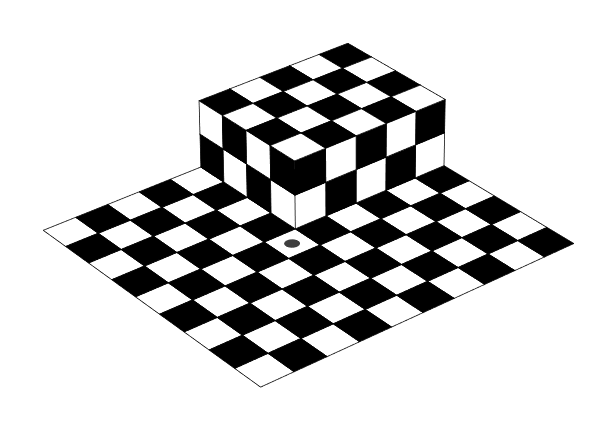
\includegraphics[width=250pt]{Images/img7.png} \\
An ant is initially on the square marked with the black dot. The ant moves across an edge from one square to an adjacent square four times and then stops. How many of the possible finishing squares are black?
\begin{tasks}(5)
\task 6
\task 8
\task 10
\task 12
\task 14
\end{tasks}
\end{problem}
%%%%%%%\answer{a)}

\begin{problem}
If some positive integers $a,b$ and $c$ satisfy $a^2+b^2 = c^2$, it follows that...
\begin{tasks2}(2)
\task $a+b > c$
\task $c$ is odd
\task $a \neq b$
\task $c$ is not divisible by $7$
\end{tasks2}
\end{problem}
%%%%%%%\answer{A and C}

\begin{problem}
There are $51$ distinct positive integers on the blackboard, none exceeding $100$. Which statements about this board must be true?
\begin{tasks2}
\task There are two consecutive numbers
\task There are two numbers differing by $50$
\task There are two numbers summing to $100$
\task There are six numbers with the same last digit
\end{tasks2}
\end{problem}
%%%%%%%\answer{A, B and D}

\begin{problem}
The expression $n^2+n+41$, for any positive integer $n$, is certainly...
\begin{tasks2}(2)
\task prime
\task bigger than $(n+1)^2$
\task odd
\task not a square
\end{tasks2}
\end{problem}
%%%%%%%\answer{C}

%%
\newpage
%%

\section{Hard}

\begin{problem}
Quirin has $4$ sticks of length $12$. He breaks exactly one of them into two sticks and arranges all five pieces to a right-angled triangle. How big is the area of that triangle?
\end{problem}
%%%%%%%\answer{96}

\begin{problem}
Let $n$ be the smallest positive integer, such that $10n$ is a square number and $6n$ is a cube number. What is $n$?
\end{problem}
%%%%%%%\answer{36000}

\begin{problem}
In how many different ways can a $2\times 11$ rectangle be filled with $11$ indistinguishable dominoes of size $1\times 2$?
\end{problem}
%%%%%%%\answer{144}

\begin{problem}
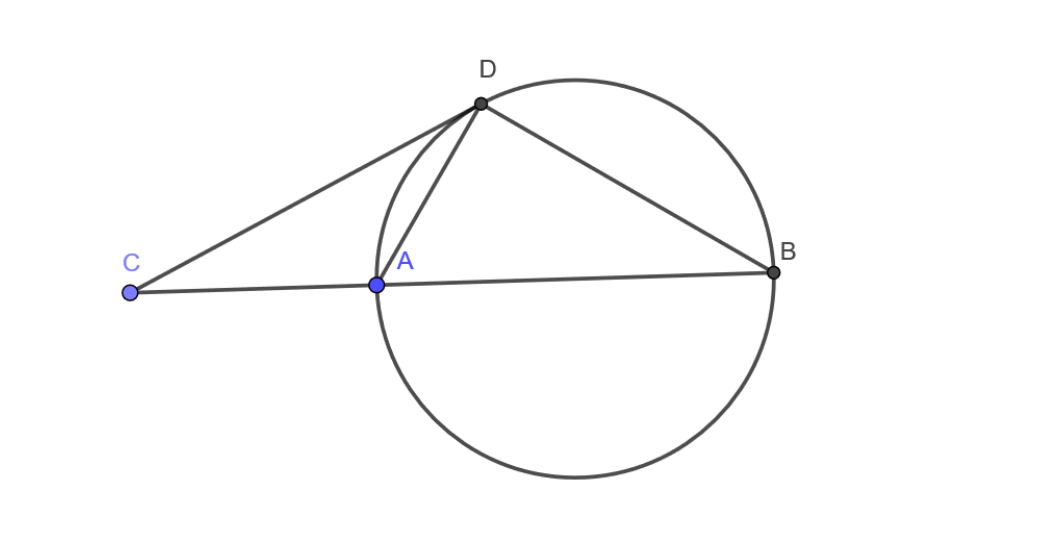
\includegraphics[width=250pt]{Images/img8.png} \\
$AB$ is the diameter of a circle, $C$ is on the line $AB$ and $CD$ is a tangent to the circle. If $|CA|=34$, $|AD|=48$ and $|DB|=90$, what is the length of $CD$?
\end{problem}
%%%%%%%\answer{68}

\newpage 

\begin{problem}
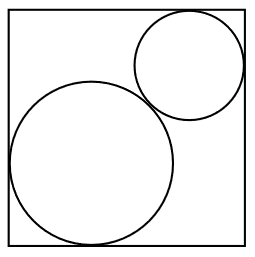
\includegraphics[width=100pt]{img3} \\
Two circles are inscribed in a square of side length $1$, as shown in the picture above. What is the sum of the two radii?
\end{problem}
\begin{tasks}(2)
\task $\dfrac{1}{2}$
\task $\dfrac{1}{\sqrt{2}}$
\task $\sqrt{2} - 1$
\task $2 - \sqrt{2}$
\task The value depends on the circles.
\end{tasks}
%%%%%%%\answer{d)}

\begin{problem}
There are $100$ coins in a line, all showing heads. Louis now turns every, then every second, then every third and so on up to every $100$th coin. Assuming that the first coin was flipped every time, how many coins show heads at the end?
\end{problem}
\begin{tasks}
\task 50
\task 89 
\task 90
\task 91
\task 99
\end{tasks}
%%%%%%%\answer{d)}

\begin{problem}
All the numbers from $1$ up to $10$ are written on the blackboard. David now repeatedly replaces two numbers by their (non-negative) difference until only one number is left. Which of the following could this number possibly be?
\begin{tasks}(5)
\task 0
\task 1
\task 4
\task 6
\task 11
\end{tasks}
%%%%%%%\answer{b)}
\end{problem}

\begin{problem}
For a given positive integer $n > 1$, we write down all its positive divisors in ascending order: \\
$1 < d_1 < \ldots < d_k < n$. How many different $n$ satisfy $d_k = 11\cdot d_1$?
\end{problem}
\begin{tasks}(5)
\task 0
\task 1
\task 2
\task 4
\task 5
\end{tasks}
%%%%%%%\answer{e)}

\begin{problem}
There exists a three-digit number $ABC$, such that
\begin{tasks2}
\task{$ABC$ is divisible by $C$ and the two-digit number $AB$}
\task{$ABC$ is divisible by $A$ and the two-digit number $BC$}
\task{$A>C>0$ and $ABC - CBA$ is a prime number} 
\task{$ABC + BCA + CAB = 2021$}
\end{tasks2}
\end{problem}
%%%%%%%\answer{A}

\begin{problem}
The five friends $A$, $B$, $C$, $D$ and $E$ are playing a social deduction game. Good guys always have to tell the truth and bad guys always have to lie. This is their conversation:
\begin{enumerate}[label=\Alph*:]
\item "C and D are either both good or both bad." 
\item "If E is good, A is telling the truth!"
\item "There is an even number of bad guys in the game."
\item "At least one among A, B and C has to be bad."
\item "A and C are not both good."
\end{enumerate}
Which of the following statements are true?
\end{problem}
\begin{tasks2}
\task It is possible that $A$ and $C$ are both good
\task $D$ is certainly good
\task $B$ is certainly bad
\task It's possible that there is only one good player
\end{tasks2}
%%%%%%%\answer{A, B, C}

\end{document}